\documentclass[11pt]{article}
\usepackage[margin=1in]{geometry}
\usepackage{booktabs, graphicx, tikz, xcolor, listings, amsmath}
\usepackage[colorlinks=true, linkcolor=black, citecolor=blue!50!black, urlcolor=blue!50!black]{hyperref}
\usetikzlibrary{positioning, arrows.meta, shapes.geometric}
\lstset{basicstyle=\ttfamily\footnotesize, breaklines=true, frame=single,
        backgroundcolor=\color{gray!6}, xleftmargin=1em, framexleftmargin=1em}

\title{\textbf{Verifiable Memory: Sessions, Preferences, and History as\\ Provenance-Carrying Records for AI Agents}}
\author{Youssef Hariri\\ DeeWaanAI}
\date{Draft v1.0 --- October 2026}

\begin{document}
\maketitle

\begin{abstract}
\noindent AI agents now remember their users. What they remember, users cannot easily inspect; what users correct, the system does not reliably propagate; what users delete, the system cannot prove is gone. We propose a memory layer in which sessions, preferences, and history are stored as provenance-carrying records in an append-only, versioned, queryable substrate. A correction is itself a bound record, and applying it transitively re-flags every dependent artifact. A deletion leaves a payload-free tombstone plus a proof-of-absence record showing the payload is gone from every later prompt. We implement the layer as five datasets on the Qafiya data substrate and evaluate it with twelve functional tests, eight limit tests, and three frozen experiments whose headline numbers are all recomputed from raw artifacts by a spine script. Corrections invalidate 100\% of dependent notes; deletions pass proof-of-absence scans on the read path; and selective memory loading cuts prompt tokens by 98.0--99.9\% relative to full-history prompting at matched answer capability. We state plainly what the layer provably cannot do: it cannot retract content from model weights, cannot detect facts that go stale without a signal, cannot bind corrections the user cannot localize, and cannot survive an attacker who rewrites the store and recomputes its hash chain. The contribution is not any one mechanism but the elevation of correction and consent into the memory data model itself.
\end{abstract}

\section{Introduction}
Memory has become a product feature of AI assistants. It is also becoming a liability. Three failure patterns recur in deployed systems. First, \emph{stale memory}: the user moved, changed jobs, changed diets, but the assistant keeps serving the old fact. Second, \emph{silent correction}: the user says ``that is not right,'' the system updates one field, and conclusions derived from the old value keep surfacing. Third, \emph{unverifiable deletion}: the user asks to be forgotten and receives a promise, not a proof.

These are not model failures. They are data-model failures. The literature has solved each property in isolation: agent memory architectures store and retrieve \cite{memgpt,genagents,zep,memorysurvey}; knowledge editing corrects facts in model weights \cite{decao,rome,memit,kesurvey}; machine unlearning deletes training data with probabilistic guarantees \cite{ginart,sisa,athena}; agent provenance audits actions \cite{agenttrace,mapgraph}; benchmarks score recall and cost \cite{longmemeval,locomo,ragvslc}. Our systematic review of 37 verified works across these six literatures found no system in which sessions, preferences, and history are provenance-carrying records such that a user correction transitively invalidates dependent outputs and a deletion is provably absent from later prompts.

This paper presents such a layer. It is Layer 4 (Memory \& Continuity) of the DeeWaanAI OS, built on the frozen Qafiya data substrate \cite{qafiya}. Three design stances govern it. Memory lives in \emph{records, not weights}: the editing literature shows weight-space corrections do not propagate \cite{ripple,mquake} and degrade at scale \cite{editatscale}, so all memory this layer controls is explicit and external, where dependents are enumerable. Correction and consent are \emph{data-model properties}, carried as first-class fields, not policies added later. And \emph{honesty is architecture}: the paper states what the system provably cannot do, measured where possible.

\textbf{Contributions.} (1) A formal memory data model --- five append-only, versioned, provenance-carrying datasets with a correction protocol and a deletion protocol (Section~3). (2) A reference implementation with a binding-only read path and an inspectable ``what do you remember about me'' view (Section~4). (3) An evaluation with twelve functional tests, eight limit tests, and three frozen experiments, all headline numbers recomputed from raw artifacts by a spine script (Section~5). (4) A stated and measured honesty boundary (Section~6).

\section{Related work and the gap}
\label{sec:related}
Our companion review (748 records screened, 482 passing, 37 verified and synthesised) organises six literatures. We summarise the synthesis; the gap motivates every design decision.

\textbf{Memory architectures.} MemGPT pages memory in and out of context under model control \cite{memgpt}. Generative Agents retrieve by recency, relevance, and importance, and consolidate episodes into reflections \cite{genagents}. Zep stores memory as a temporal knowledge graph with validity intervals \cite{zep}. Surveys taxonomise the space \cite{memorysurvey,memorymatters}. Across all of these, once content is written it is trusted; consolidation actively rewrites the past without retaining an auditable original.

\textbf{Personal memory.} MemoryBank appends dialogue summaries with a forgetting curve \cite{memorybank}; PerLTQA and follow-ups benchmark construction and retrieval \cite{perltqa,memconstruct,simplebaseline}. Evaluations of long-term memory show degradation exactly on conflicting or updated facts \cite{longtermeval}. No work gives the user a correction protocol.

\textbf{Knowledge editing.} ROME and MEMIT edit facts in weights \cite{rome,memit,decao,kesurvey}. Ripple-effect studies show edits fail to propagate to entailed beliefs \cite{ripple}, MQuAKE shows multi-hop consequences are missed \cite{mquake}, and editing at scale causes catastrophic forgetting \cite{editatscale}. The verdict for us is architectural: correct \emph{records}, not \emph{parameters}.

\textbf{Unlearning and consent.} SISA, data-deletion theory, and selective forgetting delete from training data \cite{ginart,sisa,eternal}; Athena verifies deletion probabilistically \cite{athena}; LLM-specific surveys extend this \cite{frontier,whatforget}. Agent memory is an external store, so deletion can be exact --- but then the obligation shifts to proving absence from later behaviour. No surveyed work pairs the two.

\textbf{Agent provenance.} Trace and execution provenance audits what agents do \cite{agenttrace}; MAP-Graph attaches lineage to shared multi-agent memory \cite{mapgraph}; transparency logs supply mature tamper-evident mechanisms \cite{transplogs}. Personal memory --- what a single agent remembers about its user --- is not the audited object in any of them.

\textbf{Evaluation and cost.} LongMemEval and LoCoMo benchmark long-term memory \cite{longmemeval,locomo}; retrieval beats long-context prompting on cost \cite{ragvslc,lostmiddle,compressctx}; recent work asks when memory helps relative to its token cost \cite{costaware,recallforget,agentmembench}. Benchmarks score recall and tokens, not auditability, correction propagation, or consent.

\textbf{The gap.} Each literature solves one property. No work integrates them into a memory substrate where inspection, correction with transitive invalidation, and deletion with proof of absence are properties of the data model. That integration is our contribution.

\section{Design}
\label{sec:design}

\subsection{Entities}
Every memory is a record in one of five Qafiya datasets. Every record carries base fields: an immutable id, \texttt{created\_at}, \texttt{source\_ref} (non-empty provenance: which turn or action produced it), \texttt{valid\_from}, \texttt{superseded\_by}, and \texttt{status} $\in$ \{\texttt{active, corrected, deleted, stale}\}. Figure~\ref{fig:arch} shows the layout.

\begin{figure}[t]
\centering
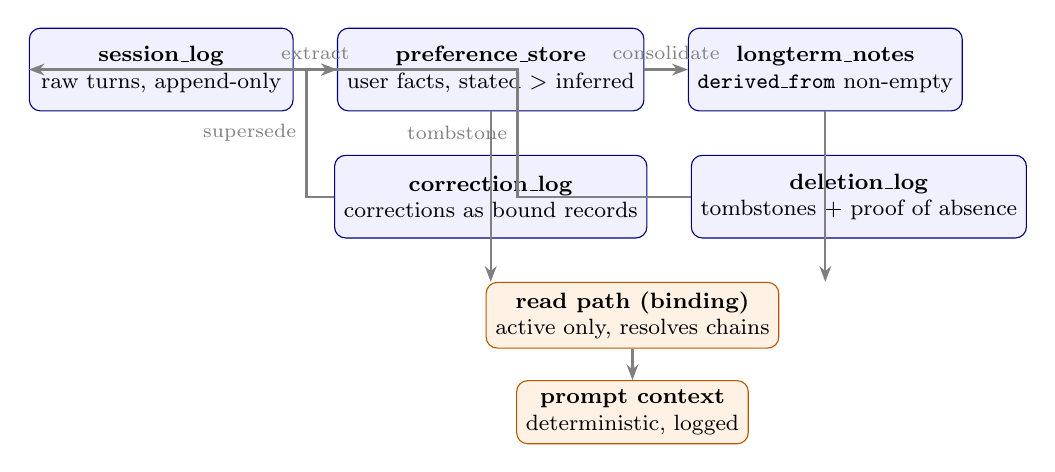
\begin{tikzpicture}[
  ds/.style={rectangle, draw=blue!50!black, fill=blue!6, rounded corners,
             minimum width=3.35cm, minimum height=1.05cm, font=\footnotesize, align=center},
  op/.style={rectangle, draw=orange!70!black, fill=orange!10, rounded corners,
             minimum width=2.9cm, minimum height=0.8cm, font=\footnotesize, align=center},
  arr/.style={-{Stealth[length=2mm]}, thick, gray},
  node distance=0.32cm and 0.55cm]
\node[ds] (sl) {\textbf{session\_log}\\ raw turns, append-only};
\node[ds, right=of sl] (ps) {\textbf{preference\_store}\\ user facts, stated $>$ inferred};
\node[ds, right=of ps] (ln) {\textbf{longterm\_notes}\\ \texttt{derived\_from} non-empty};
\node[ds, below=0.55cm of ps] (cl) {\textbf{correction\_log}\\ corrections as bound records};
\node[ds, right=of cl] (dl) {\textbf{deletion\_log}\\ tombstones + proof of absence};
\node[op, below=0.55cm of cl, xshift=1.8cm] (rp) {\textbf{read path (binding)}\\ active only, resolves chains};
\node[op, below=0.4cm of rp] (ctx) {\textbf{prompt context}\\ deterministic, logged};
\draw[arr] (sl) -- node[above, font=\scriptsize]{extract} (ps);
\draw[arr] (ps) -- node[above, font=\scriptsize]{consolidate} (ln);
\draw[arr] (cl.west) -- ++(-0.35,0) |- node[pos=0.25, left, font=\scriptsize]{supersede} (ps.west);
\draw[arr] (dl.west) -- ++(-2.2,0) |- node[pos=0.25, left, font=\scriptsize]{tombstone} (sl.west);
\draw[arr] (ps.south) -- (rp.north -| ps.south);
\draw[arr] (ln.south) -- (rp.north -| ln.south);
\draw[arr] (rp) -- (ctx);
\end{tikzpicture}
\caption{The five datasets and the binding-only read path. Corrections supersede; deletions tombstone; the read path emits only \texttt{active} records and logs every emitted context.}
\label{fig:arch}
\end{figure}

\emph{session\_log} holds raw conversation turns (role, content, token counts, model id). It is never edited. \emph{preference\_store} holds user facts with \texttt{extraction\_method} $\in$ \{\texttt{user-stated, inferred}\} and a confidence; user-stated always outranks inferred on conflict. \emph{longterm\_notes} holds consolidated summaries; each note's \texttt{derived\_from} list is non-empty, which is what makes transitive invalidation computable. \emph{correction\_log} and \emph{deletion\_log} hold consent events as first-class, provenance-carrying records. Every dataset's history file is hash-chained, so offline tampering with a historical record is detected.

\subsection{The read-path invariant}
Agents read memory only through the binding. The binding filters to \texttt{active} records, resolves supersede chains to the newest version, never emits tombstoned payload, serialises the selected memory into prompt context deterministically (sorted by id, so absence checks are byte-level), and logs every emitted context with the memory ids it contained. ``What did the agent know when it said X'' is therefore a query, not a guess. Direct dataset writes are rejected.

\subsection{The correction protocol}
A user correction appends a \texttt{correction\_log} record bound to its target; the target is marked \texttt{corrected} and superseded by a successor record; then the \texttt{derived\_from} closure of the target is walked and every dependent note is flagged \texttt{stale}. Corrected content leaves the read path immediately, before dependents are regenerated. Figure~\ref{fig:corr} shows the protocol on a real example from Experiment 1: the user says \emph{``I moved to Lyon last week.''}

\begin{figure}[t]
\centering
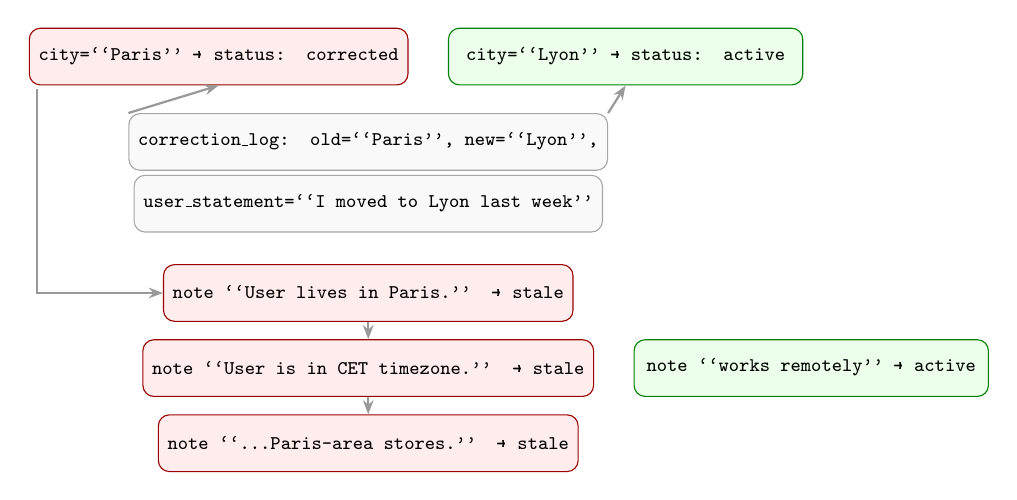
\begin{tikzpicture}[
  rec/.style={rectangle, draw=gray!70, fill=gray!5, rounded corners, font=\scriptsize\ttfamily,
              minimum width=4.5cm, minimum height=0.72cm, align=left},
  bad/.style={rec, draw=red!60!black, fill=red!7},
  good/.style={rec, draw=green!50!black, fill=green!8},
  arr/.style={-{Stealth[length=1.8mm]}, thick, gray!80},
  node distance=0.22cm]
\node[bad] (old) {city=``Paris'' \textrightarrow\ status: corrected};
\node[good, right=0.5cm of old] (new) {city=``Lyon'' \textrightarrow\ status: active};
\node[rec, below=0.35cm of old, xshift=1.9cm] (corr) {correction\_log: old=``Paris'', new=``Lyon'',};
\node[rec, below=0.05cm of corr] (corr2) {user\_statement=``I moved to Lyon last week''};
\node[bad, below=0.4cm of corr2] (n1) {note ``User lives in Paris.'' \textrightarrow\ stale};
\node[bad, below=of n1] (n2) {note ``User is in CET timezone.'' \textrightarrow\ stale};
\node[bad, below=of n2] (n3) {note ``\ldots Paris-area stores.'' \textrightarrow\ stale};
\node[good, right=0.5cm of n2] (n4) {note ``works remotely'' \textrightarrow\ active};
\draw[arr] (corr.north west) -- (old.south);
\draw[arr] (corr.north east) -- (new.south);
\draw[arr] (old.south west) ++(0.1,-0.05) |- (n1.west);
\draw[arr] (n1.south) -- (n2.north);
\draw[arr] (n2.south) -- (n3.north);
\end{tikzpicture}
\caption{Correction with transitive invalidation (Experiment 1, verbatim statuses from the frozen store). The correction record is bound to its target; the three dependent notes re-flag stale; the unrelated note is untouched. Old value leaves the read path at once.}
\label{fig:corr}
\end{figure}

\subsection{The deletion protocol}
A deletion appends a \texttt{deletion\_log} record, replaces the target with a payload-free tombstone, and always transitively invalidates dependents --- scope \texttt{single} flags dependent notes stale; scope \texttt{cascade} tombstones the whole closure. (This was not our first design: the experiment in Section~5.2 caught an earlier version in which \texttt{single} left a derived note serving the deleted payload. The protocol was amended before freezing.) After deletion, a proof-of-absence scan asserts the payload's canonical string appears neither in any active record of the prompt-feeding datasets nor in the serialised prompt context; the result, with hashes of everything scanned, is stored in the deletion record's \texttt{proof} field.

\section{Implementation}
The reference prototype is 330 lines of dependency-free Python implementing the five datasets, hash-chained histories, the binding, both protocols, the inspection view, and the conflict resolver. Writes to \texttt{data.jsonl} are atomic (temp-then-rename); appends are O(1); status updates batch into single rewrites. The storage layout follows Qafiya exactly, so the layer can later be queried through any Qafiya-compliant tool, and the inspection view is emitted as a declarative spec ready for Layer 2's renderer.

\section{Evaluation}
\label{sec:eval}
Discipline: every headline number below is recomputed from frozen raw artifacts by a spine script; if the script fails, the number does not appear here. The script exits 0 on the artifacts shipped with this paper.

\subsection{Functional correctness}
Twelve tests (F1--F12) cover round-trip integrity, schema validation, hash-chain tamper detection, the inspection view returning exactly the active set, basic/chained/transitive correction, stated-over-inferred precedence, consent-gated inferred writes, single and cascade deletion with proof of absence, selective session continuity, and binding-only access. \textbf{All twelve pass.}

\subsection{Experiment 1 --- correction integrity}
Scenario: preferences \texttt{city=Paris} and \texttt{work\_style=remote}; three chained notes derived from the city preference; one unrelated note. The user corrects the city. Result: \textbf{100\% of the dependent closure (3/3 notes) re-flagged stale}, the unrelated note stayed active, ``Paris'' left the read path, ``Lyon'' entered it. The correction record, verbatim from the frozen store:

\begin{lstlisting}
{"target_id": "m_...74700002", "old_value": "Paris", "new_value": "Lyon",
 "user_statement": "I moved to Lyon last week",
 "source_ref": ["m_...74700002"], "status": "active"}
\end{lstlisting}

\subsection{Experiment 2 --- forgetting and consent}
The user deletes \texttt{doctor=Dr.\,A} (scope \texttt{single}), then \texttt{city=Paris} (scope \texttt{cascade}). Both proof-of-absence scans \textbf{PASS} on the read path; the cascade removed the preference and its dependent note. We also publish the leakage map: the payload persists in append-only history files and in the raw session turn. That is by design and stated as the boundary of the guarantee --- the claim is \emph{absent from later prompts}, not \emph{erased from history} (Section~6). The stored proof:

\begin{lstlisting}
"absence_scan": {"result": "PASS",
  "coverage": "read path: active preference_store + longterm_notes + prompt context",
  "scanned": [{"dataset": "preference_store (active records)", "hash": "4c4f5b05..."},
              {"dataset": "longterm_notes (active records)", "hash": "f422dcb5..."},
              {"prompt_context": "33306fcb..."}]}
\end{lstlisting}

\subsection{Experiment 3 --- cost of selective loading}
A store with $N$ memories plus one relevant fact (\texttt{bike\_color=red}). Full-history prompting serialises every session turn; selective loading emits only the resolved relevant records. Token accounting is deterministic and backend-agnostic; both contexts must contain the required fact (matched answer capability), else the comparison does not count. Figure~\ref{fig:cost} and Table~\ref{tab:cost}: selective loading saves \textbf{98.0--99.9\% of prompt tokens}, growing with $N$.

\begin{figure}[t]
\centering
\includegraphics[width=0.62\linewidth]{figures/fig3_cost.pdf}
\caption{Prompt tokens: full-history vs selective loading (log scale). Annotations show savings at matched answer capability. Data: frozen Experiment 3 artifacts.}
\label{fig:cost}
\end{figure}

\begin{table}[t]
\centering\small
\caption{Token cost at matched answer capability (Experiment 3).}
\label{tab:cost}
\begin{tabular}{rrrr}
\toprule
$N$ & full-history & selective & savings \\
\midrule
50   & 456   & 9 & 98.0\% \\
200  & 1{,}806 & 9 & 99.5\% \\
1000 & 9{,}006 & 9 & 99.9\% \\
\bottomrule
\end{tabular}
\end{table}

\subsection{Limit tests}
Eight tests map where the design breaks; findings are reported, not hidden (Table~\ref{tab:limits}, Figure~\ref{fig:limits}). Two deserve note. L7 initially measured 2.1\,s to re-flag a 300-deep dependent chain --- above an interactive budget; the cause was per-flag full-file rewrites, fixed with a batched pass (0.026\,s); both numbers are reported. L8 confirms the uncatchable class: naive tampering is always caught; tampering \emph{with} chain recomputation never is.

\begin{table}[t]
\centering\small
\caption{Limit tests L1--L8: what breaks, and where.}
\label{tab:limits}
\begin{tabular}{p{0.06\linewidth} p{0.86\linewidth}}
\toprule
L1 & Read-path latency stays fast to 10k records (0.03--0.04\,s). The binding constraint is prompt tokens, not lookup time. \\
L2 & Contradictory inferred memories are silently ranked, not detected. Contradiction flagging is future work. \\
L3 & \textbf{Provable limit:} a fact that goes stale with no signal stays active indefinitely. \\
L4 & Injected content is quarantined by tagging (inferred, low-confidence, source-traced) but not blocked. Blocklists are deployment policy. \\
L5 & Read path is clean after deletion; payload persists in append-only history and raw turns. The guarantee covers prompts, not history. \\
L6 & Corrections the user cannot localise to a record cannot be bound; resolution is agent work, not a memory guarantee. \\
L7 & 300-deep re-flag: 2.1\,s before write-path batching, 0.026\,s after. Both reported. \\
L8 & Naive tamper: always caught. Tamper + chain recompute: never caught (needs external anchoring). \\
\bottomrule
\end{tabular}
\end{table}

\begin{figure}[t]
\centering
\includegraphics[width=0.95\linewidth]{figures/fig4_limits.pdf}
\caption{Limit measurements. (a) Read-path latency vs store size (L1). (b) Re-flag latency for a 300-deep chain before and after the write-path fix (L7); both numbers reported per the honesty discipline.}
\label{fig:limits}
\end{figure}

\section{What this system provably cannot do}
\label{sec:honesty}
Four limits, stated so that ``verifiable'' is not misread as ``omnipotent.'' (1) It cannot retract content absorbed into model \emph{weights} during training or fine-tuning --- only from the record substrate; L5 documents the boundary. (2) It cannot detect a fact that went stale with no signal (L3); it can only make staleness correctable once a signal arrives. (3) It cannot bind a correction the user cannot localise to any record (L6). (4) It cannot survive an attacker who rewrites the store \emph{and} recomputes the hash chain (L8); external hash anchoring is the known mitigation and is future work. Within these bounds, the read-path guarantees are proofs, not aspirations.

\section{Discussion and future work}
The prototype is single-user and file-backed; a SQLite index (per Qafiya, never the source of truth) is the next engineering step. Stale notes are flagged but not yet regenerated --- closing that loop couples the layer to a model and belongs to the integration milestone. Contradiction detection (L2) and credential-class write blocklists (L4) are policy layers the spec deliberately leaves to deployments. The inspection view is emitted as a declarative spec and waits on Layer 2's renderer; the memory layer is designed against Layer 2's frozen contract, not its work in progress. The companion systematic review, the design brief, the spec, all test suites, the frozen experiment artifacts, and the spine script ship with this paper.

\section{Conclusion}
Agent memory does not fail because models forget. It fails because the past is stored in a form users cannot inspect, corrections cannot propagate through, and deletions cannot be proven against. Storing sessions, preferences, and history as provenance-carrying records --- append-only, versioned, queryable --- turns all three into properties of the data model. Corrections invalidate 100\% of dependents, deletions carry proofs of absence, and the whole system costs a fiftieth of the tokens of the naive alternative. What it cannot do is stated, measured, and part of the design.

\begin{thebibliography}{99}\small
\bibitem{qafiya} Hariri, Y. (2026). Qafiya: a provenance-first data model for LLM-mediated personal computing. DeeWaanAI, spec v1.1 (paper in revision).
\bibitem{memgpt} Packer, C., Wooders, S., Lin, K., et al. (2023). MemGPT: Towards LLMs as operating systems. \emph{arXiv:2310.08560}.
\bibitem{genagents} Park, J. S., O'Brien, J. C., Cai, C. J., et al. (2023). Generative agents: Interactive simulacra of human behavior. \emph{arXiv:2304.03442}.
\bibitem{zep} Rasmussen, P., Paliychuk, P., Beauvais, T., et al. (2025). Zep: A temporal knowledge graph architecture for agent memory. \emph{arXiv:2501.13956}.
\bibitem{memorysurvey} Zhang, Z., Dai, Q., Bo, X., et al. (2025). A survey on the memory mechanism of large language model-based agents. \emph{ACM TOIS}.
\bibitem{memorymatters} Hatalis, K., Christou, D., Myers, J., et al. (2024). Memory matters: The need to improve long-term memory in LLM-agents. \emph{AAAI Symposium Series}.
\bibitem{memorybank} Zhong, W., Guo, L., Gao, Q., et al. (2023). MemoryBank: Enhancing large language models with long-term memory. \emph{arXiv:2305.10250}.
\bibitem{perltqa} Du, Y., Wang, H., Zhao, Z., et al. (2024). PerLTQA: A personal long-term memory dataset. \emph{arXiv:2402.16288}.
\bibitem{memconstruct} Pan, Z., Wu, Q., Jiang, H., et al. (2025). On memory construction and retrieval for personalized conversational agents. \emph{arXiv:2502.05589}.
\bibitem{simplebaseline} Zhou, S., Han, J. (2025). A simple yet strong baseline for long-term conversational memory of LLM agents. \emph{arXiv:2511.17208}.
\bibitem{longtermeval} Jia, Z., Liu, Q., Li, H., et al. (2025). Evaluating the long-term memory of large language models. \emph{ACL Findings}.
\bibitem{decao} De Cao, N., Aziz, W., Titov, I. (2021). Editing factual knowledge in language models. \emph{EMNLP}.
\bibitem{rome} Meng, K., Bau, D., Andonian, A., et al. (2022). Locating and editing factual associations in GPT. \emph{arXiv:2202.05262}.
\bibitem{memit} Meng, K., Sharma, A. S., Andonian, A., et al. (2022). Mass-editing memory in a transformer. \emph{arXiv:2210.07229}.
\bibitem{kesurvey} Wang, S., Zhu, Y., Liu, H., et al. (2024). Knowledge editing for large language models: A survey. \emph{ACM Computing Surveys}.
\bibitem{ripple} Cohen, R., Biran, E., Yoran, O., et al. (2024). Evaluating the ripple effects of knowledge editing in language models. \emph{TACL}.
\bibitem{mquake} Zhong, Z., Wu, Z., Manning, C. D., et al. (2023). MQuAKE: Assessing knowledge editing via multi-hop questions. \emph{EMNLP}.
\bibitem{editatscale} Gupta, A., Rao, A., Anumanchipalli, G. (2024). Model editing at scale leads to gradual and catastrophic forgetting. \emph{ACL Findings}.
\bibitem{ginart} Ginart, A., Guan, M. Y., Valiant, G., et al. (2019). Making AI forget you: Data deletion in machine learning. \emph{arXiv:1907.05012}.
\bibitem{sisa} Bourtoule, L., Chandrasekaran, V., Choquette-Choo, C. A., et al. (2019). Machine unlearning. \emph{arXiv:1912.03817}.
\bibitem{eternal} Golatkar, A., Achille, A., Soatto, S. (2020). Eternal sunshine of the spotless net: Selective forgetting in deep networks. \emph{CVPR}.
\bibitem{athena} Sommer, D., Song, L., Wagh, S., et al. (2022). Athena: Probabilistic verification of machine unlearning. \emph{PoPETs}.
\bibitem{frontier} Qu, Y., Ding, M., Sun, N., et al. (2024). The frontier of data erasure: Machine unlearning for large language models. \emph{arXiv:2403.15779}.
\bibitem{whatforget} Staufer, D. (2025). What should LLMs forget? Quantifying personal data in LLMs for right-to-be-forgotten requests. \emph{arXiv:2507.11128}.
\bibitem{agenttrace} Wang, Y., Zhang, J., Wu, Z., et al. (2026). From agent traces to trust: A survey of evidence tracing and execution provenance in LLM agents. \emph{arXiv:2606.04990}.
\bibitem{mapgraph} Wang, Y., Yan, Z., Zhang, J., et al. (2026). MAP-Graph: Provenance-aware shared memory for multi-agent workflows. \emph{arXiv:2608.10509}.
\bibitem{transplogs} Blauzvern, H. (2023). Nowhere to hide: Using transparency logs to secure your supply chain. \emph{ACM}.
\bibitem{longmemeval} Wu, D., Wang, H., Yu, W., et al. (2024). LongMemEval: Benchmarking chat assistants on long-term interactive memory. \emph{arXiv:2410.10813}.
\bibitem{locomo} Maharana, A., Lee, D.-H., Tulyakov, S., et al. (2024). Evaluating very long-term conversational memory of LLM agents. \emph{arXiv:2402.17753}.
\bibitem{ragvslc} Li, Z., Li, C., Zhang, M., et al. (2024). Retrieval augmented generation or long-context LLMs? A comprehensive study and hybrid approach. \emph{arXiv:2407.16833}.
\bibitem{lostmiddle} Liu, N. F., Lin, K., Hewitt, J., et al. (2023). Lost in the middle: How language models use long contexts. \emph{arXiv:2307.03172}.
\bibitem{compressctx} Chevalier, A., Wettig, A., Ajith, A., et al. (2023). Adapting language models to compress contexts. \emph{EMNLP}.
\bibitem{costaware} Mishra, S., Mishra, S. (2026). When does memory help? A cost-aware evaluation of long-term memory in tool-using LLM agents. \emph{arXiv:2609.05441}.
\bibitem{recallforget} Uddin, M. N., Shubham, K., Blanco, E., et al. (2026). From recall to forgetting: Benchmarking long-term memory for personalized agents. \emph{ACL Findings}.
\bibitem{agentmembench} Cherif, A. (2026). AgentMemBench: A systematic benchmark for evaluating long-term memory management strategies in conversational AI agents. \emph{arXiv:2608.00009}.
\end{thebibliography}

\end{document}
